\begin{figure*}[htbp]
    \centering
    \begin{subfigure}
        {0.48\textwidth}
        \centering
        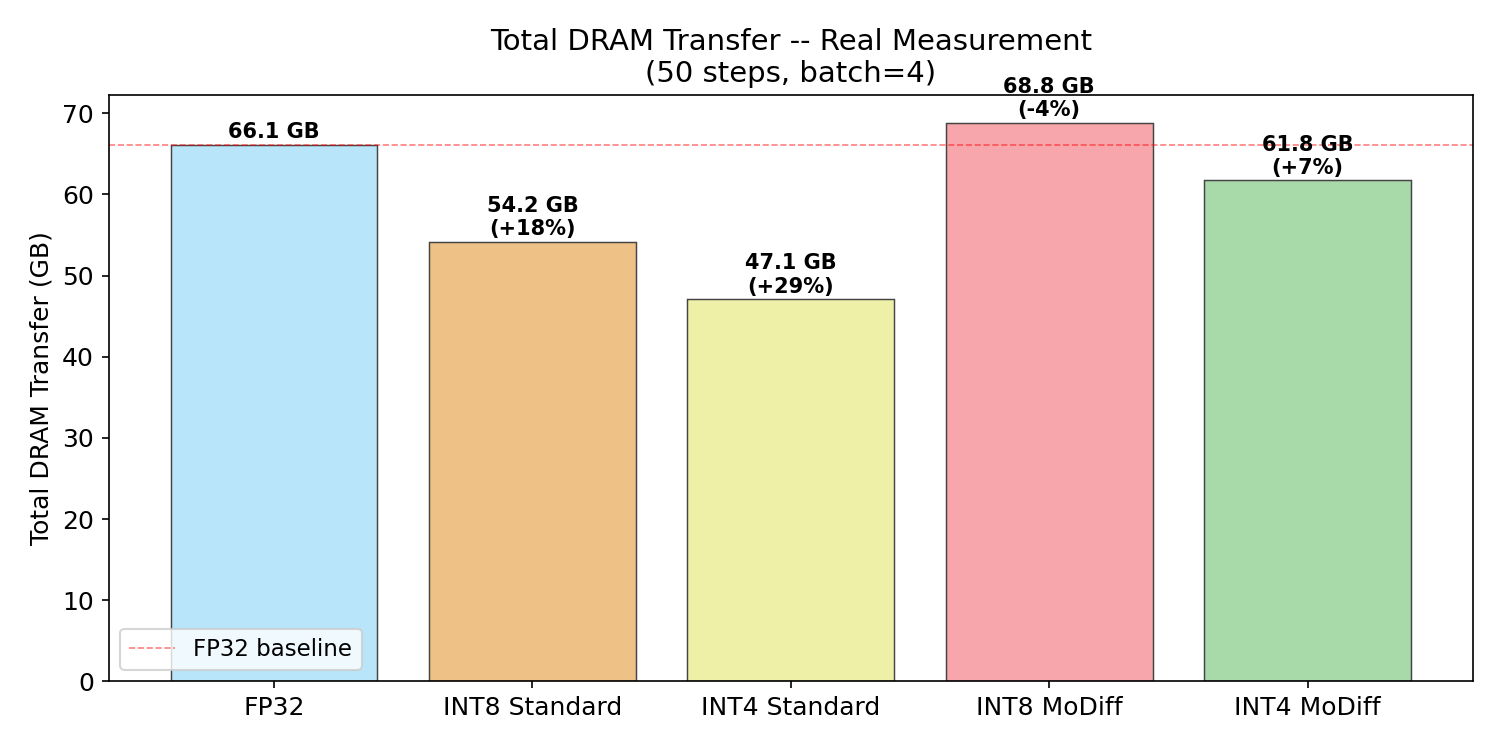
\includegraphics[width=\textwidth]{figures/plot_memory_total_io.png}
        \caption{Total HBM I/O per mode}
        \label{fig:plot_memory_total_io}
    \end{subfigure}
    \hfill
    \begin{subfigure}
        {0.48\textwidth}
        \centering
        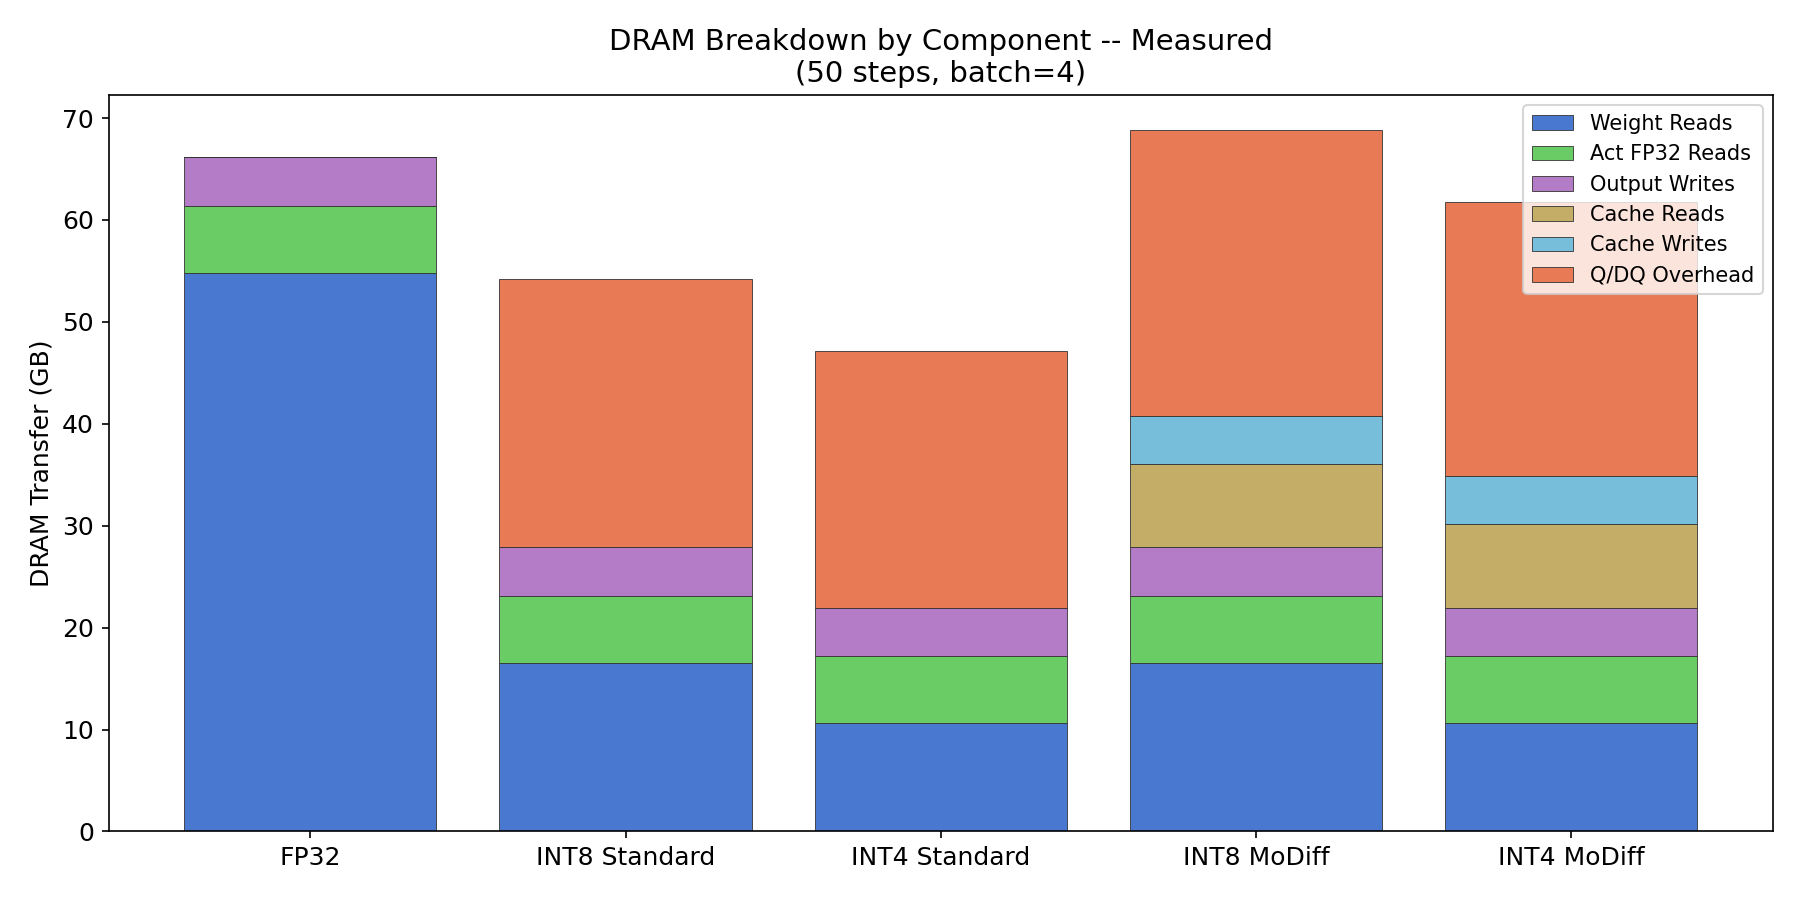
\includegraphics[width=\textwidth]{figures/plot_memory_breakdown.png}
        \caption{Stacked component breakdown}
        \label{fig:plot_memory_breakdown}
    \end{subfigure}
    \caption{Memory transfer overview: total HBM I/O (left) and per-component stacked breakdown (right) across quantization modes.}
    \label{fig:plot_memory_row1}
\end{figure*}

\begin{figure*}[htbp]
    \centering
    \begin{subfigure}
        {0.48\textwidth}
        \centering
        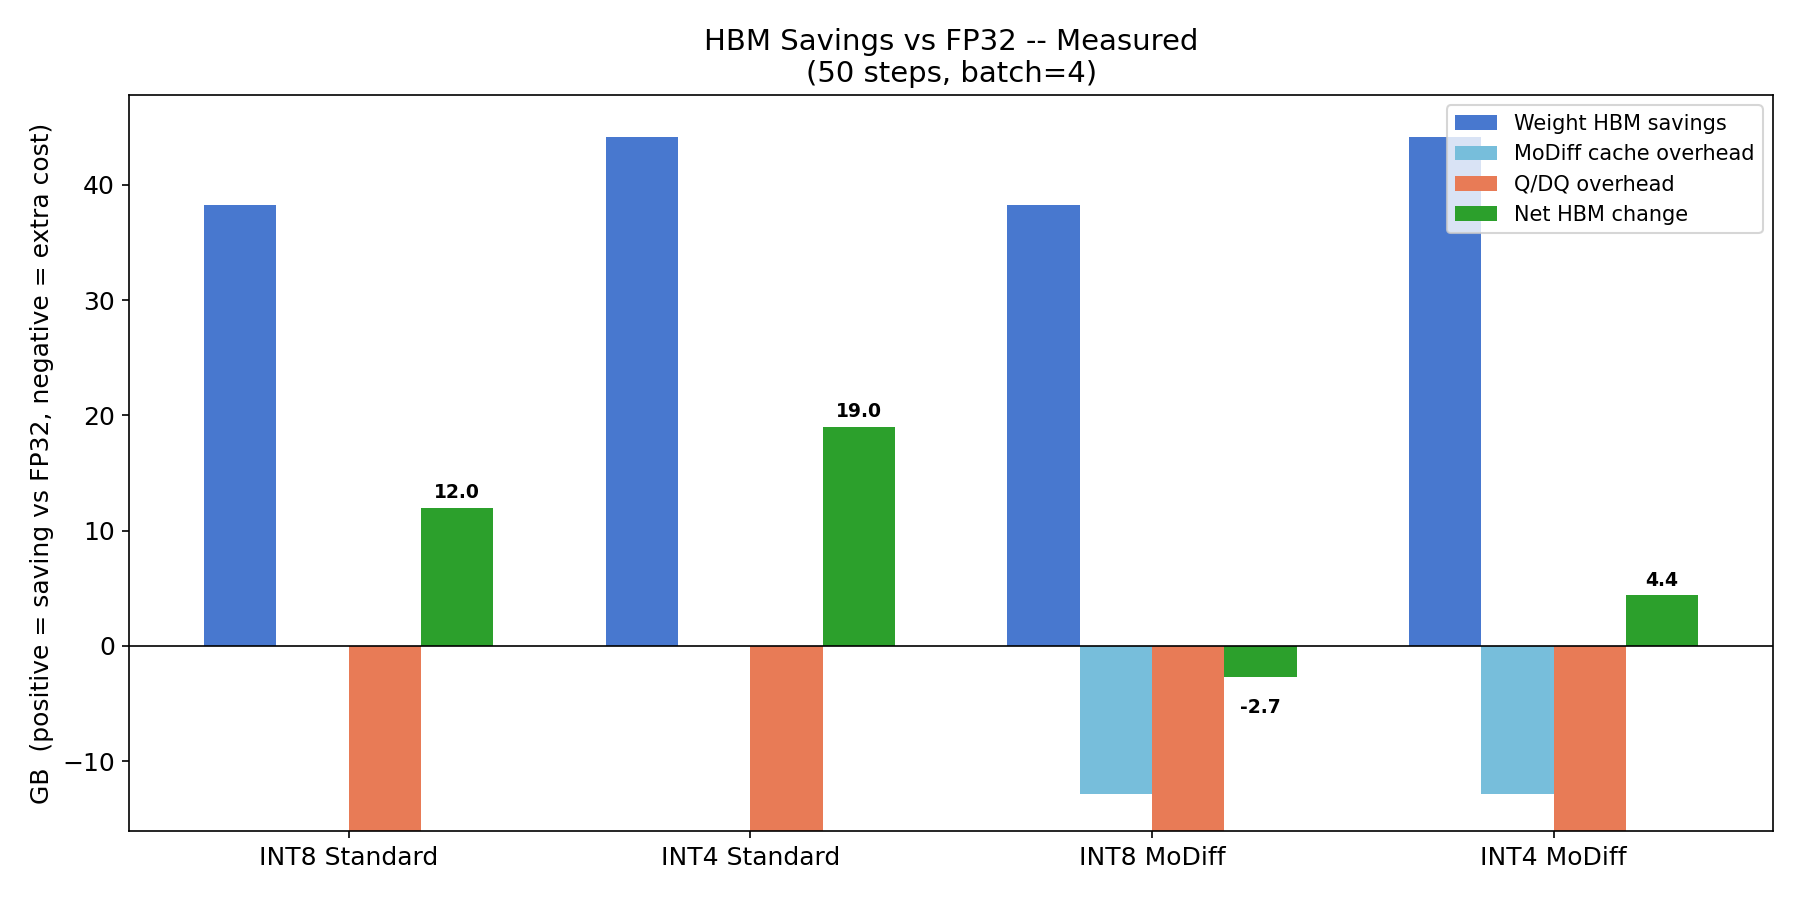
\includegraphics[width=\textwidth]{figures/plot_memory_savings.png}
        \caption{HBM savings vs.\ FP32}
        \label{fig:plot_memory_savings}
    \end{subfigure}
    \hfill
    \begin{subfigure}
        {0.48\textwidth}
        \centering
        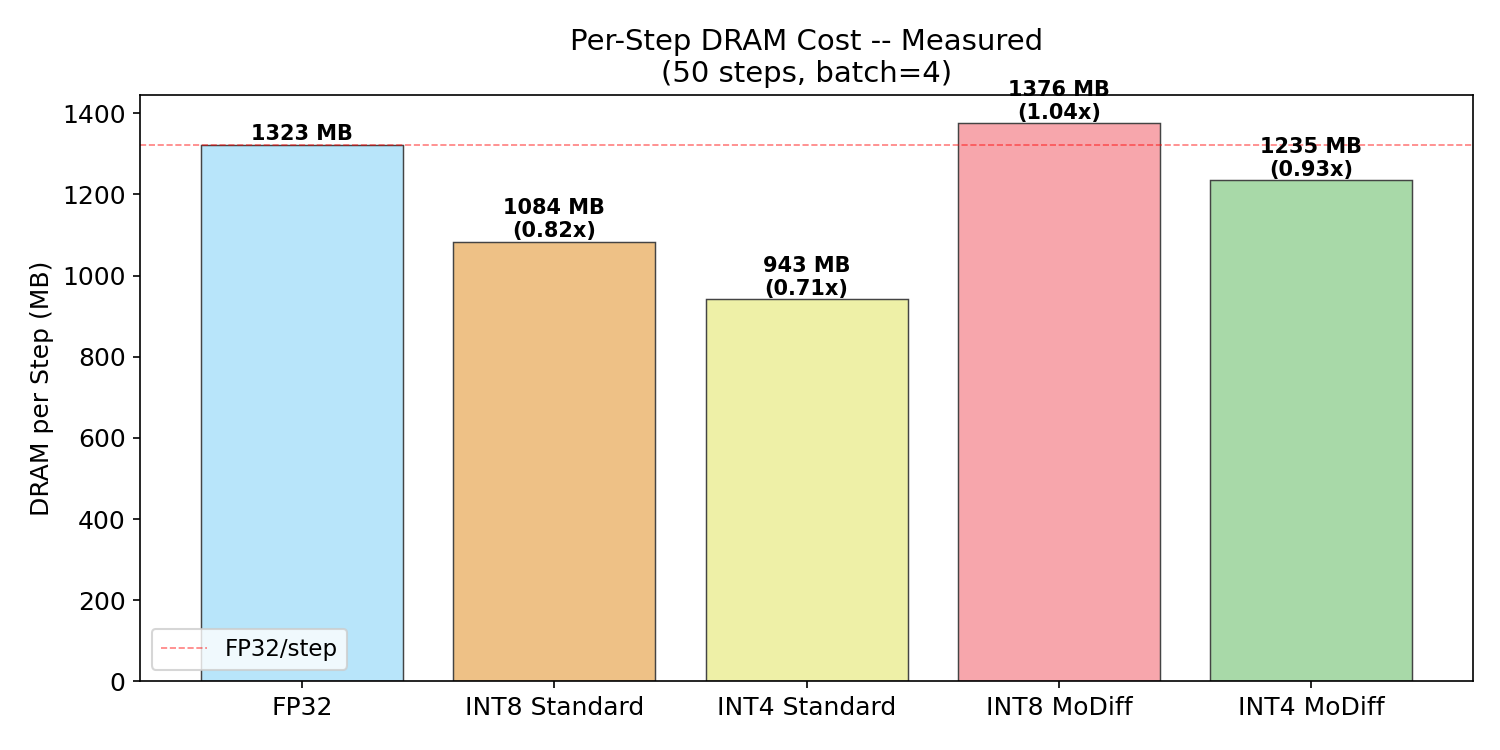
\includegraphics[width=\textwidth]{figures/plot_memory_per_step.png}
        \caption{Cumulative I/O over denoising timesteps}
        \label{fig:plot_memory_cumulative}
    \end{subfigure}
    \caption{Memory transfer dynamics: bandwidth savings relative to FP32 (left) and cumulative I/O accumulation over 50 denoising steps (right).}
    \label{fig:plot_memory_row2}
\end{figure*}